%% This is file `sample-sigconf.tex',
%% generated with the docstrip utility.
%%
%% The source files were:
%%
%% samples.dtx  (with options: `sigconf')
% TODO: Change to review before submitting
\documentclass[sigconf]{acmart}
%% \BibTeX command to typeset BibTeX logo in the docs
\AtBeginDocument{%
  \providecommand\BibTeX{{%
    \normalfont B\kern-0.5em{\scshape i\kern-0.25em b}\kern-0.8em\TeX}}}

%% Rights management information.  This information is sent to you
%% when you complete the rights form.  These commands have SAMPLE
%% values in them; it is your responsibility as an author to replace
%% the commands and values with those provided to you when you
%% complete the rights form.
\setcopyright{acmcopyright}
\copyrightyear{2024}
\acmYear{2024}
\acmDOI{XXXXXXX.XXXXXXX}

\acmConference[ICSE 2024]{46th International Conference on Software Engineering}{April 2024}{Lisbon, Portugal}

% My packages
\usepackage[nameinlink]{cleveref} % Reference footnotes.
% My packages end

%%
%% end of the preamble, the start of the body of the document source.
\begin{document}

%%
%% The "title" command has an optional parameter,
%% allowing the author to define a "short title" to be used in page headers.
\title{Implementing the visual debugger: Past, Present, and Future}
% Alternative titles
% Implementing the visual debugger: Past, Present, and Future
% Implementing the visual debugger: Past, An experience report
% Something regarding IDE integration?

\author{Tim Kr\"{a}uter}
\email{tkra@hvl.no}
\orcid{0000-0003-1795-0611}
\affiliation{
  \institution{Western Norway University of Applied Sciences}
  \city{Bergen}
  \country{Norway}
}

\author{Adrian Rutle}
\email{aru@hvl.no}
\orcid{0000-0002-4158-1644}
\affiliation{
  \institution{Western Norway University of Applied Sciences}
  \city{Bergen}
  \country{Norway}
}

% \author{Harald K\"{o}nig}
% \email{harald.koenig@fhdw.de}
% \orcid{0000-0001-6304-6311}
% \affiliation{
%   \institution{University of Applied Sciences, FHDW}
%   \city{Hannover}
%   \country{Germany}}
% \affiliation{
%   \institution{Western Norway University of Applied Sciences}
%   \city{Bergen}
%   \country{Norway}
% }

\author{Yngve Lamo}
\email{yla@hvl.no}
\orcid{0000-0001-9196-1779}
\affiliation{
  \institution{Western Norway University of Applied Sciences}
  \city{Bergen}
  \country{Norway}
}

\author{Patrick Stünkel}
\email{patrick.stuenkel@hvl.no}
\orcid{0000-0002-0537-295X}
\affiliation{
  \institution{Western Norway University of Applied Sciences}
  \city{Bergen}
  \country{Norway}
}

\renewcommand{\shortauthors}{Kräuter et al.}
\newcommand{\intellij}{IntelliJ IDEA} % <-- Space has to be there
% Four pages + 1 page of references.

%%
%% The abstract is a short summary of the work to be presented in the
%% article.
\begin{abstract}
  TODO: Abstract.
\end{abstract}

\keywords{Debugging, Visual Debugging, Plugin, IDE, IDE Integration}

% Fitting topics from the workshop:
% 1. The development of plugins, add-ons, and extensions for IDEs.
% 2. Visualizations in the IDEs.
% 3. Anecdotal experience about why a certain tool or research approach was not implemented on top of the IDE infrastructure, but researchers chose alternatives (e.g., a CLI tool), what the blockers were, and how the IDEs can improve to become more convenient for prototyping.

\received{7 December 2023}
% \received[revised]{7 December 2023}
% \received[accepted]{11 January 2024}

\maketitle

\section{Introduction}
% Context about the tool --> More high-level, do not repeat too much regarding section 2.
This paper details the experience of implementing the visual debugger \cite{krauterVisualDebuggerTool2022}.
The tool is available for \intellij{} and Android studio as a plugin \cite{timkrauterVisualDebuggerIntelliJ2023}, but its architecture makes it easily adaptable to other Integrated Development Environments (IDEs) \cite{krauterVisualDebuggerTool2022}.

% Motivation for this report?
% Roadblocks hampering full IDE integration: Swing, Tradeoff tight integration and reusability
% Implementing for more IDEs and standard debugging protocols
% Open problems due to IDE integration: Performance?

% Paper outline
The remainder of this paper is structured as follows.
We describe the visual debugger tool in detail (\cref{sec:visualDebugger}) and outline the lessons we learned and roadblocks we encountered in \cref{sec:lessonsLearned}.
Finally, we discuss related work in \cref{sec:relatedWork} and conclude in \cref{sec:conclusion}.


\section{The visual debugger} \label{sec:visualDebugger}
% What can the tool do?
The visual debugger is an open-source \intellij{} plugin that visualizes the debugging variables as an object diagram to foster program comprehension.
It is available for \intellij{} and Android Studio through the JetBrains Marketplace \cite{timkrauterVisualDebuggerIntelliJ2023, timkrauterVisualDebuggerTool2023} making use of the IntelliJ Platform \cite{kurbatovaIntelliJPlatformFramework2021}.
Our plugin was integrated into \intellij{}, the Java IDE with the highest popularity, with approximately 70\% market share as per the JVM Ecosystem Report 2021 \cite{brianvermeerJVMEcosystemReport2021}.

% Motivation
Debugging information might not be present in the top-level variables and has to be obtained by digging multiple levels (following links to related objects) deep into different variables.
Thus, in specific scenarios, especially when data is hierarchically structured, a graphical representation results in a faster and better understanding of the debugging information \cite{krauterVisualDebuggerTool2022}.

% Feedback for the tool and current vs previous downloads.
Until now, we have only received positive feedback regarding the visual debugger, which now has over 7200 downloads\footnote{Last checked on the 28th of November, 2023, see \cite{timkrauterVisualDebuggerIntelliJ2023}.}.
This marks a twofold increase in downloads compared to the initial release of our research paper \cite{krauterVisualDebuggerTool2022} on July 21, 2022, which garnered approximately 2700 downloads.

Additional artifacts, including source code, a demonstration of the visual debugger tool, and a description of the Visual Debugging API, can be found in \cite{timkrauterICSE2024Artifacts2023}.

\subsection{Description}

Traditionally, debugging information is represented textually, such as in \autoref{fig:variablesIntellij}, which shows a screenshot of the debugging variables view in \intellij.

\begin{figure}[h]
    \centering
    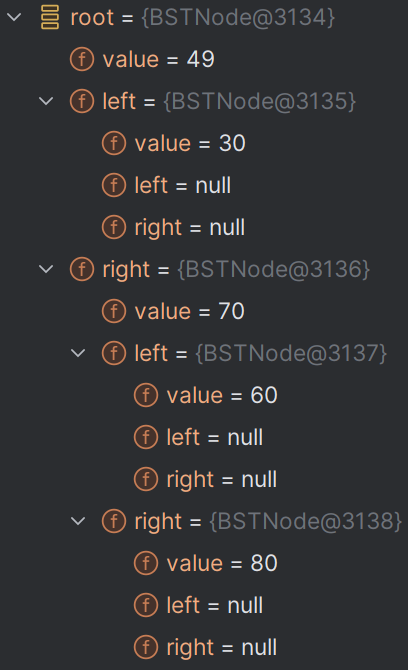
\includegraphics[width=0.4\textwidth]{images/variables.png}
    \caption{Variables during debugging in \intellij}
    \label{fig:variablesIntellij}
\end{figure}

The visual debugger will represent the same information graphically as an object diagram.
Using the visual debugger is \textit{straightforward} since it becomes available automatically during debugging in the IDE.
After activating the visual debugger, it continuously visualizes the variables in the scope of the debugging session (see, for example, \autoref{fig:variablesVisualDebugger}).
\autoref{fig:variablesVisualDebugger} contains the same objects and level of detail as \autoref{fig:variablesIntellij}.
There is a little more debug information in \autoref{fig:variablesIntellij} due to well-written \textsf{toString()} methods which are used by \intellij{}.
In addition, the coloring in \autoref{fig:variablesVisualDebugger} highlights variable changes and additions, a new feature of the visual debugger discussed in \autoref{subsec:improvements}.

\begin{figure}[ht]
    \centering
    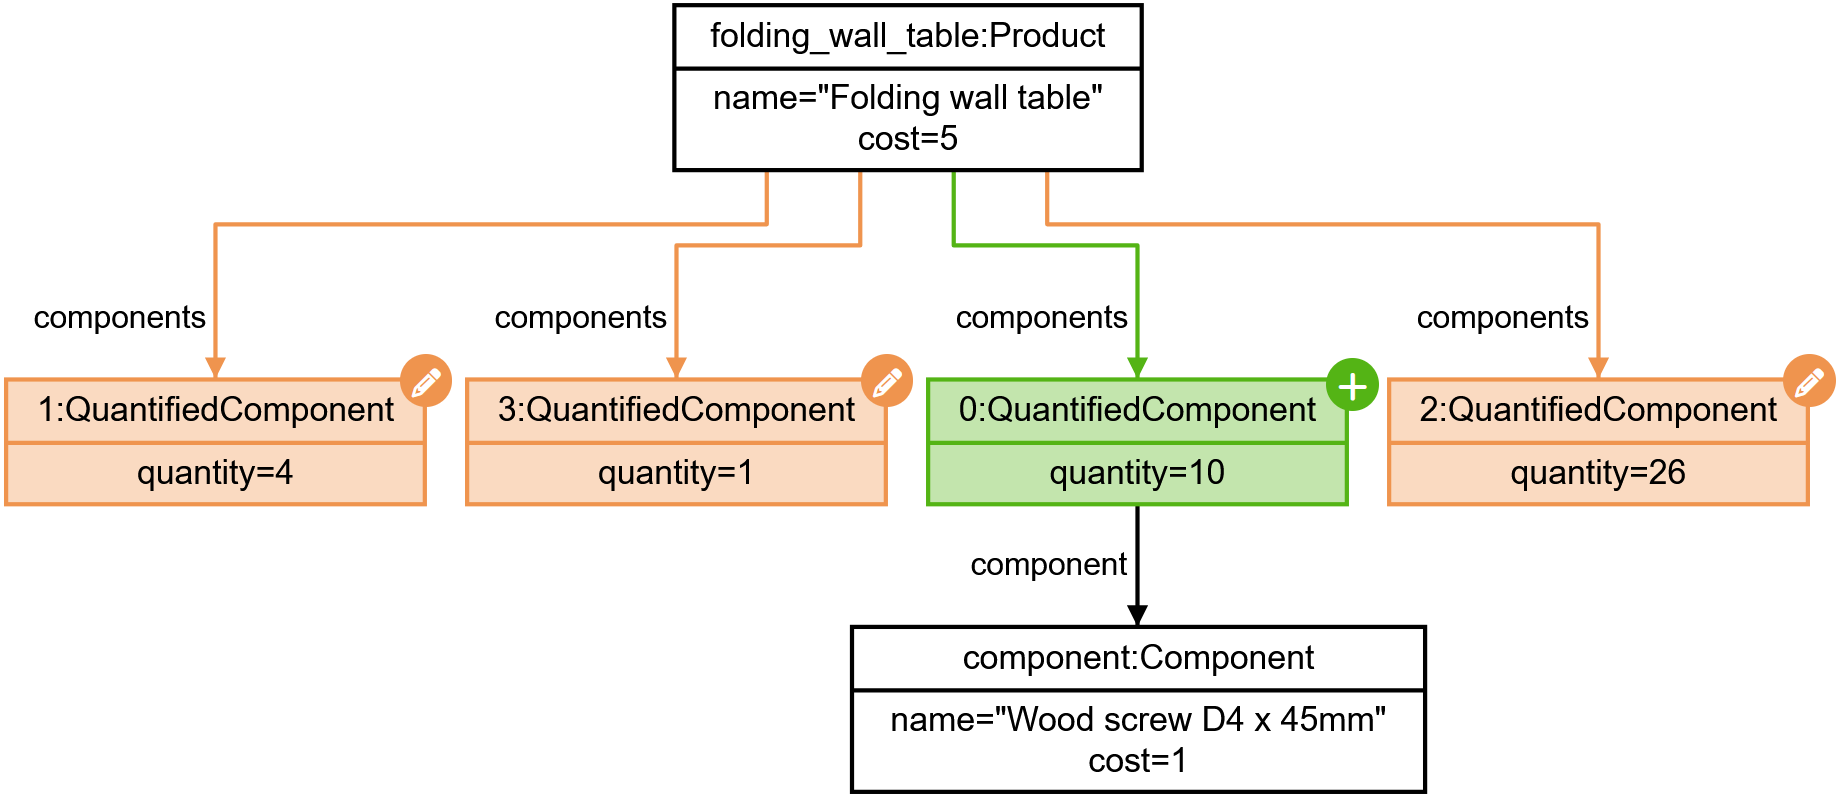
\includegraphics[width=0.475\textwidth]{images/variables-visual-debugger.png}
    \caption{Visual debugger visualization comparable to \cref{fig:variablesIntellij}}
    \label{fig:variablesVisualDebugger}
\end{figure}

The graphical visualization does not replace the textual debugging view but aims to improve program comprehension during debugging\cite{krauterVisualDebuggerTool2022}.
Concretely, the visual debugger is \textit{non-intrusive} since it can be used alongside the traditional textual debugging available in the IDE.

The visual debugger automatically updates the debug information just as the \intellij{} debugger whenever a user steps through the source code or a new breakpoint is reached.
Moreover, children of a debugging variable can be loaded by double-clicking an object in the object diagram, similar to how it works in most textual debuggers.
For example, in \autoref{fig:variablesVisualDebugger}, all children of the green object were loaded.
The goal is to make the visual debugger \textit{familiar} by adopting how textual debuggers work such that a transition is smooth.
% Minimalistic: Less is more --> Not adopt all features since this doesn't make sense.

More information about the visual debugger, including a typical usage scenario, can be found in \cite{krauterVisualDebuggerTool2022}.
% TODO: Make video 2.0 and update link.
In addition, a demonstration of the visual debugger is available at \url{https://www.youtube.com/watch?v=lU_OgotweRk}, and the tool can be installed using \cite{timkrauterVisualDebuggerIntelliJ2023}.

\subsection{Architecture}
% Structure into two components --> Important for new features and roadblocks later.
In this section, we briefly recap the architecture of the visual debugger.
% The architecture plays an important role in the new features of the visual debugger and helps us understand the roadblocks we have encountered during development.
The visual debugger is separated into two independent components communicating through the \textit{Visual Debugging API} \cite{krauterVisualDebuggerTool2022}.
\autoref{fig:architecture} summarizes the architecture of the visual debugger.

\begin{figure}[ht]
  \centering
  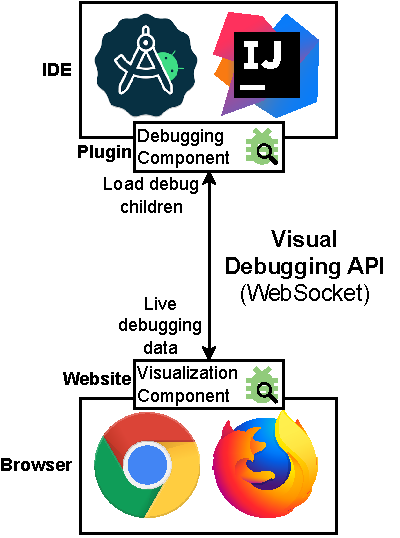
\includegraphics[width=0.8\linewidth]{images/visual-debugger-architecture.pdf}
  \caption{Visual debugger architecture}
  \label{fig:architecture}
\end{figure}

The first component, the \textit{debugging component} integrates with \intellij{}, and its primary function is to acquire and refresh debugging information throughout the debugging process.
The debugging component makes this information available via a WebSocket server that implements our Visual Debugging API.
Upon establishing a connection to the Visual Debugging API, a client receives real-time updates with the latest debugging data and can request to load children for an existing object.

The second component, the \textit{visualization component}, portrays debugging information as an object diagram for better understanding (refer to \autoref{fig:variablesVisualDebugger} for an illustration).
It is implemented using web technologies and our object diagram library \cite{timkrauterObjectdiagramjs2023} to visualize the debug information.
Additionally, it leverages the Visual Debugging API to communicate with the debugging component.
Thus, it is agnostic of the IDE used for debugging and can even be reused for other programming languages than Java/Kotlin.
In practice, the visualization component is hosted on a web server as part of the visual debugger plugin.

The downside to this flexibility is that the visual debugger is not entirely integrated into \intellij{}, as the visualization occurs in a browser external to the IDE.
The rationale behind opting for this approach instead of full integration is discussed in \autoref{sec:lessonsLearned}.

% Improvements would be better loading
\subsection{Improvements \& New Features} \label{subsec:improvements}
A major improvement under the hood of the visual debugger is how debugging information is loaded.
Previously, we had to pre-load and cache more debug information than was requested by the user since we could not load debug information on demand.
The initial load invalidated the underlying stack frame supplied by the Java Debugging Interface (JDI).
Now, we leverage the APIs provided by \intellij{}, which are a thin wrapper around the JDI.
This enables us to defer loading additional debug information until explicitly required.
Consequently, there is no longer a need to pre-load potentially unnecessary debug information.
This optimization has improved performance, making the visual debugger applicable to more intricate debugging scenarios.

Furthermore, we enhanced the visual debugger by introducing the following two new features:

% Visualizing changes
\textbf{(1)} The visualization component of the visual debugger now \textit{highlights changes} using colors and overlays in the object diagram.
New objects and links are colored green, while changes to existing elements lead to orange coloring.
Computing and highlighting the changes is enabled by default but can be switched off.
\autoref{fig:variablesVisualDebugger} shows the new change visualization by highlighting three changed, and one added object accordingly.
% Motivation
A software engineer is usually most interested in the changes that occur to the objects during debugging.
Our color-based visualization of changes in the object diagram makes it easier for a software engineer to see changes even when dealing with a complex debugging situation with multiple connected objects.

% Implementation
Changes can be calculated efficiently using unique object IDs provided during debugging.
We implemented the change detection in the visualization component such that it can be reused across programming languages and IDEs \cite{timkrauterICSE2024Artifacts2023}.

% Debug history
\textbf{(2)} Furthermore, the visualization component now keeps a \textit{debug history} so that a user can see debug information from previous debugging steps.
The debug history's length is configurable or can be turned off entirely.
% Motivation
As described earlier, software engineers are most interested in how variables change during debugging.
Consequently, to not only highlight differences to the previous step, we save the previous debugging information in a debug history.
% TODO: Potentially even step forward!
A software engineer can thus inspect the previously shown debug information and step as far back as he configured.
The visual debugger always shows where the debug information was collected in the source code, and highlights changes compared to the previous debugging step.
In addition, one can still export the debug information to an image or even edit it in our object diagram modeler \cite{timkrauterObjectdiagramjs2023} for documentation purposes \cite{krauterVisualDebuggerTool2022}.

% Implementation
We implemented the \textit{debug history} in the visualization component to be independent of the used programming language and IDE.
Thus, both features follow our aim of providing a reusable visualization of the debugging information set in our previous publication \cite{krauterVisualDebuggerTool2022}.
% Smarter UI?. Shows if more information is available (colors and icons). --> Colors and overlays can be adapted from BPMN-js

\section{Lessons Learned \& Roadblocks} \label{sec:lessonsLearned}

% Roadblock 1: IDE integration due to IDE UI technology --> See notes

% Roadblock 2: Missing APIS
% \subsection{IDE APIs}
% Is the Go plugin not possible due to the lack of APIs? --> Access to the APIs needed to integrate plugins with the IDE deeply. Deeper integration means less portability (to other ideas) but a better user experience.
% Or it is possible, but the integration would not be nice! Since now, we have two people connected to the same process or something similar.
% Possible Solution DAP!
DAP \cite{microsoftDebugAdapterProtocol2023}

sibling of LSP \cite{microsoftLanguageServerProtocol2023}

Related citations:
\cite{jeanjeanIDECodeReifying2021,raskVisualStudioCode2020,borkLanguageServerProtocol2023}

% Should also mention strong points: Forum with quick and helpful answers. For example, our debugging loading. --> One lessons learned ask precise detailed questions including your problem setting in the forum after investigating yourself

\section{Related work} \label{sec:relatedWork}

\section{Conclusion \& Future work} \label{sec:conclusion}
% Conclusion

% Summarize stats of the plugin --> Interest in other languages such as GoLang
% Summarize new features
% Summarize roadblocks and lessons learned

% Summarize the design principles of the debugger: non-invasive, familiar? -> no surprises, i.e., predictable, intuitive behavior, simple (less is more)


% Future work
Implement for other IDEs and code editors such as Eclipse \cite{desrivieresEclipsePlatformIntegrating2004} and Visual Studio Code.

% This summary could lead to the following empirical studies:
% 1. Empirical study about the usability of the tool
% 2. Does the visual debugger boost productivity in certain scenarios? Which scenarios? If yes, how much is the productivity boosted?

% Add acknowledgments after review
% \section{Acknowledgments}

\bibliographystyle{ACM-Reference-Format}
\bibliography{bib}
\end{document}
